% Este archivo es parte de la memoria del proyecto fin de carrera
% de Manuel López Urbina. Protegida bajo la licencia GFDL.
% Para más información, la licencia completa viene incluida en el
% fichero fdl-1.3.tex

% Copyright (C) 2012 Manuel López Urbina

\chapter{Anexos}
\label{chap:anexos}

\section{Instalación de OpenCV}

El siguiente anexo indica la instalación de OpenCV 2.4.1 en Ubuntu 12.04 LTS.\\

La presente guía de instalación detalla los pasos para instalación de OpenCV con la nueva interfaz Qt highgui, que ofrece muchas más funcionalidades que la sencilla interfaz highgui. Además, se procederá a la instalación de OpenCV con soporte para OpenGL, así como vídeos de lectura y escritura, el acceso a una cámara web, Python, C y C++ interfaz, e Intel Threading Building Blocks (TBB).\\

Previamente hay que asegurarse de que todo en el sistema está actualizado:\\

\begin{lstlisting}[style=consola]
sudo apt-get update
sudo apt-get upgrade
\end{lstlisting}

A continuación se deben instalar muchas dependencias y secos como soporte para leer y escribir archivos de imagen, dibujar en la pantalla, algunas herramientas necesarias, etc. Para ello introducimos en la terminal terminal:\\

\begin{lstlisting}[style=consola]
sudo apt-get install build-essential libgtk2.0-dev libjpeg-dev libtiff4-dev libjasper-dev libopenexr-dev cmake python-dev python-numpy python-tk libtbb-dev libeigen2-dev yasm libfaac-dev libopencore-amrnb-dev libopencore-amrwb-dev libtheora-dev libvorbis-dev libxvidcore-dev libx264-dev libqt4-dev libqt4-opengl-dev sphinx-common texlive-latex-extra libv4l-dev libdc1394-22-dev libavcodec-dev libavformat-dev libswscale-dev !/bin/bash
\end{lstlisting}

A continuación descargamos el código fuente de OpenCV 2.4.1:\\

\begin{lstlisting}[style=consola]
cd ~
wget http://downloads.sourceforge.net/project/opencvlibrary/opencv-unix/ 2.4.1/OpenCV-2.4.1.tar.bz2
tar -xvf OpenCV-2.4.1.tar.bz2
cd OpenCV-2.4.1
\end{lstlisting}

Ahora tenemos que generar el Makefile usando cmake. De aquí podemos definir qué partes de OpenCV queremos compilar. Como queremos usar Python, TBB, OpenGL, Qt, el trabajo con vídeos, etc, aquí es donde tenemos que establecer eso. Simplemente ejecute la ayuda en línea en la terminal para crear el makefile apropiado. Tenga en cuenta que hay dos puntos al final de la línea, es un argumento para el programa cmake y significa el directorio padre (porque estamos dentro del directorio de construcción, y queremos hacer referencia al directorio de OpenCV, que es su padre ).\\

\begin{lstlisting}[style=consola]
mkdir build
cd build
cmake -D WITH_TBB=ON -D BUILD\_NEW\_PYTHON\_SUPPORT=ON -D WITH_V4L=ON -D INSTALL\_C\_EXAMPLES=ON -D INSTALL\_PYTHON\_EXAMPLES=ON -D BUILD\_EXAMPLES=ON -D WITH\_QT=ON -D WITH\_OPENGL=ON ..
\end{lstlisting}

Compruebe que el comando anterior produce ningún error y que en particular aparece FFMPEG como S. Si no está activado no será capaz de visualizar vídeos. Asimismo, compruebe que Python, TBB, OpenGL, V4L, OpenGL y Qt son detectados. Ver figura \ref{figura:opencv-ok}.\\

\begin{figure}[H]
  \begin{center}
    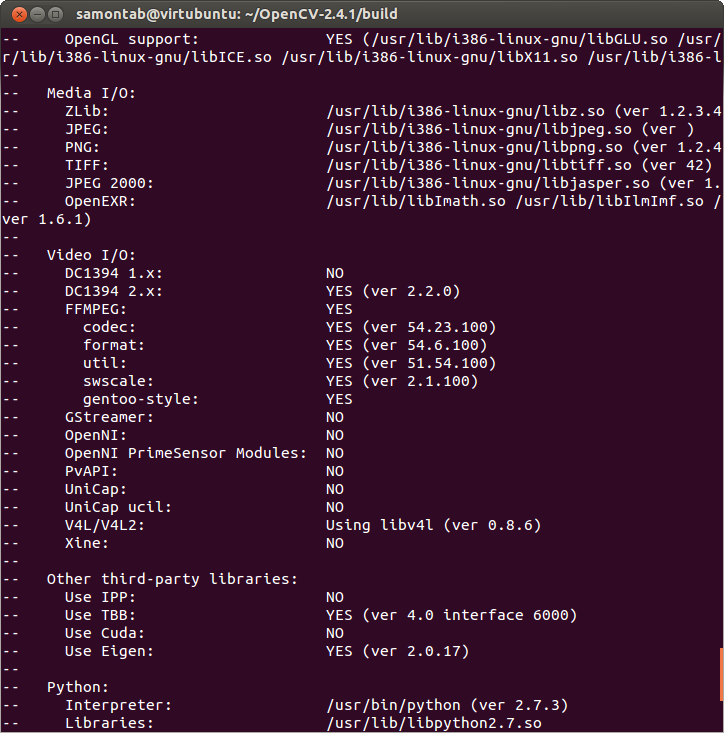
\includegraphics[scale=0.5]{opencv-ok.png}
  \end{center}
  \caption{Chequeo de la configuración de OpenCV.}
  \label{figura:opencv-ok}
\end{figure}

Si algún elemento anterior aparece como desactivado, revise los pasos anteriores y corrija los errores mediante la instalación de paquetes adicionales. Revise de nuevo la configuración tras la ejecución nuevamente de cmake.\\

Pasado este punto, todo está listo para compilar e instalar OpenCV 2.4.1:\\

\begin{lstlisting}[style=consola]
make
sudo make install
\end{lstlisting}

Ahora tienes que configurar OpenCV. En primer lugar, abrir el archivo opencv.conf con la siguiente orden:\\

\begin{lstlisting}[style=consola]
sudo gedit /etc/ld.so.conf.d/opencv.conf
\end{lstlisting}

Agregue la siguiente línea al final del archivo y guarde los cambios:\\

\begin{lstlisting}[style=consola]
/Usr/local/lib
\end{lstlisting}

Ejecute el siguiente comando para configurar la biblioteca:\\

\begin{lstlisting}[style=consola]
sudo ldconfig
\end{lstlisting}

Ahora se debe editar otro archivo:\\

\begin{lstlisting}[style=consola]
sudo gedit /etc/bash.bashrc
\end{lstlisting}

Se añaden estas dos líneas al final del archivo. Guarde los cambios:\\

\begin{lstlisting}[style=consola]
PKG\_CONFIG\_PATH=\$PKG\_CONFIG\_PATH:/usr/local/lib/pkgconfig
export PKG\_CONFIG\_PATH
\end{lstlisting}

Por último, reinicie el equipo o cierre la sesión e inicie nuevamente. OpenCV no funcionará correctamente hasta que lo haga.\\

Llegado a este punto OpenCV 2.4.1 está instalado en su ordenador con Python, TBB, OpenGL, video y soporte Qt.\\

El siguiente paso es opcional aunque se recomienda para comprobar que todo se ha instalado correctamente. Para ello se va a compilar algunos de los ejemplos proporcionados por OpenCV:\\

\begin{lstlisting}[style=consola]
cd ~/OpenCV-2.4.1/samples/c
chmod +x build\_all.sh
./build\_all.sh
\end{lstlisting}

Una vez compilados se procede a ejecutar los ejemplos:\\

\begin{lstlisting}[style=consola]
./facedetect --cascade="/usr/local/share/OpenCV/haarcascades
/haarcascade\_frontalface\_alt.xml" --nested-cascade="/usr/local/share
/OpenCV/haarcascades/haarcascade\_eye.xml" --scale=1.5 lena.jpg
\end{lstlisting}

\begin{figure}[H]
  \begin{center}
    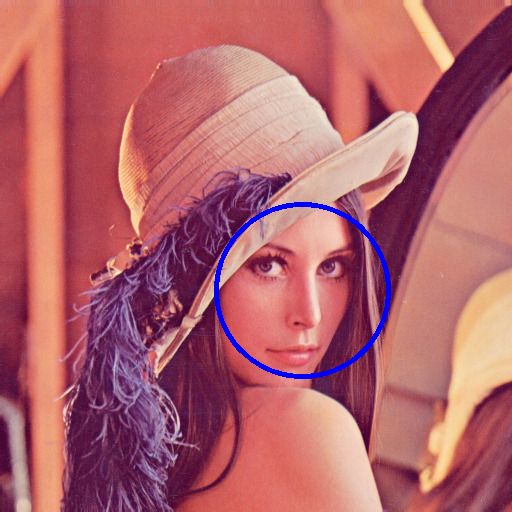
\includegraphics[scale=0.5]{lenaSample.png}
  \end{center}
  \caption{Salida producida tras la ejecución del programa de ejemplo.}
  \label{subsistemas}
\end{figure}

\section {Instalación Qt y Qt Creator}

El SDK de Qt incluye las herramientas que necesarias para la elaboración de interfaces gráficas compatibles con multitud de dispositivos como ordenadores de escritorio y móviles entre otros. Todas las herramientas necesarias se encuentran incorporadas en este instalador. \\

Como paso previo a la instalación se debe descargar el instalador del siguiente enlace http://qt.nokia.com/downloads/. Se recomienda la descarga del instalador offline, en el caso de esta guía se explica el proceso de instalación de la versión para Linux 64 bits. El resto de las versiones no difiere demasiado.\\

Una vez descargado el instalador, se procede con la instalación.\\

En sistemas Linux/Unix, es necesario asignar permisos para la ejecución del instalador. Para asignar permisos de ejecución previamente identificado como administrador y en una terminal, escriba:\\

\begin{lstlisting}[style=consola]
chmod u + x Qt\_SDK\_Lin64\_offline\_v1\_2\_en.run
\end{lstlisting}

Ahora debería ser capaz de ejecutar el archivo. Para su ejecución, desde la línea de comandos, escriba:\\

\begin{lstlisting}[style=consola]
./Qt\_SDK\_Lin64\_offline\_v1\_2\_en.run
\end{lstlisting}

A continuación se muestra la ventana de bienvenida del instalador, pulsamos en \emph{Next}.\\

\begin{figure}[H]
  \begin{center}
    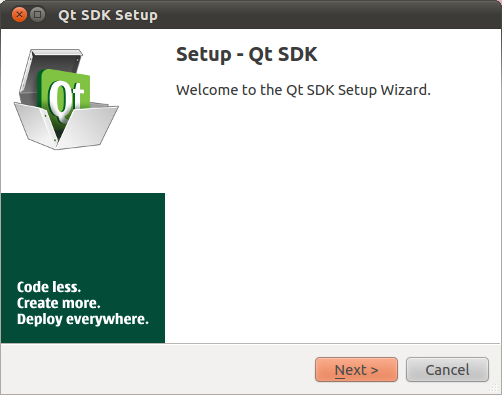
\includegraphics[scale=0.5]{QtSDKSetup-1.png}
  \end{center}
  \caption{Ventana de bienvenida del instalador.}
  \label{opencv-ok}
\end{figure}

La siguiente ventana solicita el establecimiento de la rutas de instalación, se dejan valores por defecto.\\

\begin{figure}[H]
  \begin{center}
    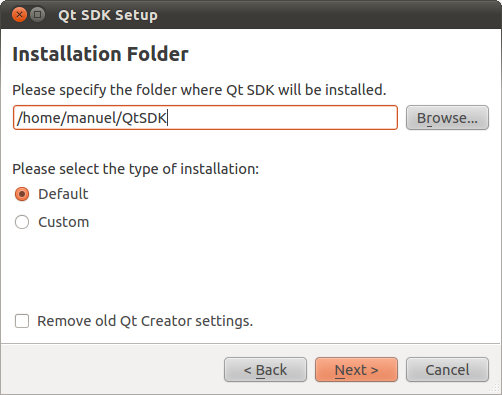
\includegraphics[scale=0.5]{QtSDKSetup-2.png}
  \end{center}
  \caption{Solicitud de directorio para la instalación.}
  \label{opencv-ok}
\end{figure}

En la nueva ventana aceptamos los términos de licencia y pulsamos sobre \emph{Next}.\\

\begin{figure}[H]
  \begin{center}
    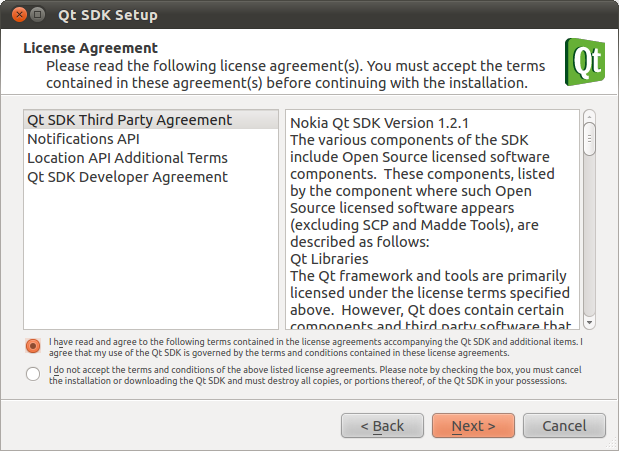
\includegraphics[scale=0.5]{QtSDKSetup-3.png}
  \end{center}
  \caption{Ventana para la visualización de los términos de licencia.}
  \label{opencv-ok}
\end{figure}

Finalmente, ya introducida toda la configuración, pulsamos sobre el botón \emph{Install} para proceder con la instalación. \\

\begin{figure}[H]
  \begin{center}
    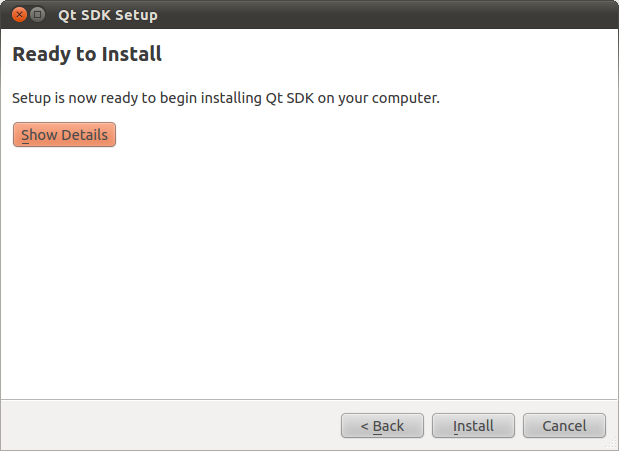
\includegraphics[scale=0.5]{QtSDKSetup-4.png}
  \end{center}
  \caption{Ventana de comienzo de instalación.}
  \label{opencv-ok}
\end{figure}

Se espera durante unos minutos a que se complete el proceso de instalación. \\

\begin{figure}[H]
  \begin{center}
    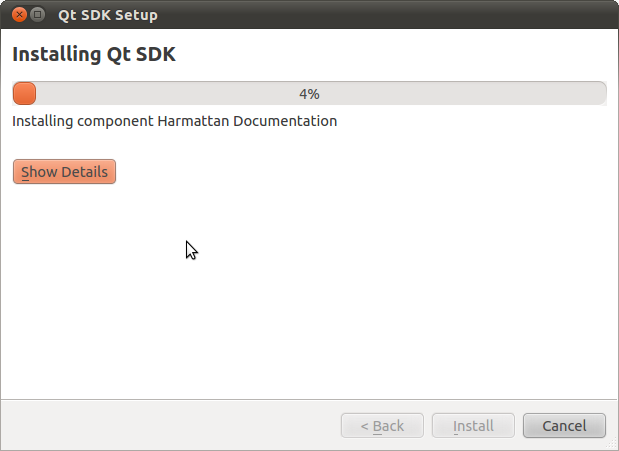
\includegraphics[scale=0.5]{QtSDKSetup-5.png}
  \end{center}
  \caption{Proceso de instalación de Qt SDK.}
  \label{opencv-ok}
\end{figure}


Llegados a este punto disponemos de la aplicación Qt SDK instalada. Pulsamos en \emph{Finish}.\\

\begin{figure}[H]
  \begin{center}
    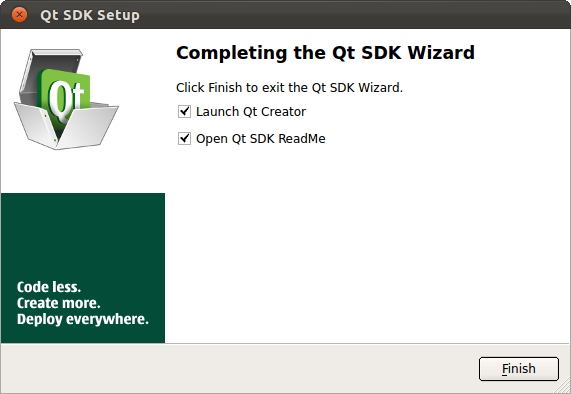
\includegraphics[scale=0.5]{qt-ultima.png}
  \end{center}
  \caption{Proceso de instalación finalizado.}
  \label{opencv-ok}
\end{figure}

\section{Instalación de SDL}

Los paquetes necesarios se encuentran disponible en el repositorio universe, por tanto es recomendable proceder a su instalación desde terminal. Los paquetes necesarios son los siguientes:

\begin{itemize}
\item libsdl1.2debian.
\item libsdl1.2-dev.
\item libsdl-image1.2.
\item libsdl-image1.2-dev.
\item libsdl-mixer1.2.
\item libsdl-mixer1.2-dev.
\item libsdl-ttf1.2.
\item libsdl-ttf1.2-dev.
\end{itemize}

Para la instalación de los citados paquetes, introducimos en una terminal:\\

\begin{lstlisting}[style=consola]
sudo apt-get install libsdl1.2debian libsdl1.2-dev libsdl-image1.2 libsdl-image1.2-dev libsdl-mixer1.2 libsdl-mixer1.2-dev libsdl-ttf1.2 libsdl-ttf1.2-dev
\end{lstlisting}

Una vez completado el proceso de instalación dispondremos de los diferentes elementos que incorpora esta biblioteca.\\
